% Options for packages loaded elsewhere
\PassOptionsToPackage{unicode}{hyperref}
\PassOptionsToPackage{hyphens}{url}
%
\documentclass[
  a4paper,
]{article}
\usepackage{lmodern}
\usepackage{amssymb,amsmath}
\usepackage{ifxetex,ifluatex}
\ifnum 0\ifxetex 1\fi\ifluatex 1\fi=0 % if pdftex
  \usepackage[T1]{fontenc}
  \usepackage[utf8]{inputenc}
  \usepackage{textcomp} % provide euro and other symbols
\else % if luatex or xetex
  \usepackage{unicode-math}
  \defaultfontfeatures{Scale=MatchLowercase}
  \defaultfontfeatures[\rmfamily]{Ligatures=TeX,Scale=1}
\fi
% Use upquote if available, for straight quotes in verbatim environments
\IfFileExists{upquote.sty}{\usepackage{upquote}}{}
\IfFileExists{microtype.sty}{% use microtype if available
  \usepackage[]{microtype}
  \UseMicrotypeSet[protrusion]{basicmath} % disable protrusion for tt fonts
}{}
\makeatletter
\@ifundefined{KOMAClassName}{% if non-KOMA class
  \IfFileExists{parskip.sty}{%
    \usepackage{parskip}
  }{% else
    \setlength{\parindent}{0pt}
    \setlength{\parskip}{6pt plus 2pt minus 1pt}}
}{% if KOMA class
  \KOMAoptions{parskip=half}}
\makeatother
\usepackage{xcolor}
\IfFileExists{xurl.sty}{\usepackage{xurl}}{} % add URL line breaks if available
\IfFileExists{bookmark.sty}{\usepackage{bookmark}}{\usepackage{hyperref}}
\hypersetup{
  pdftitle={MATH2750 Introduction to Markov Processes},
  pdfauthor={Matthew Aldridge},
  hidelinks,
  pdfcreator={LaTeX via pandoc}}
\urlstyle{same} % disable monospaced font for URLs
\usepackage[margin=1in]{geometry}
\usepackage{longtable,booktabs}
% Correct order of tables after \paragraph or \subparagraph
\usepackage{etoolbox}
\makeatletter
\patchcmd\longtable{\par}{\if@noskipsec\mbox{}\fi\par}{}{}
\makeatother
% Allow footnotes in longtable head/foot
\IfFileExists{footnotehyper.sty}{\usepackage{footnotehyper}}{\usepackage{footnote}}
\makesavenoteenv{longtable}
\usepackage{graphicx,grffile}
\makeatletter
\def\maxwidth{\ifdim\Gin@nat@width>\linewidth\linewidth\else\Gin@nat@width\fi}
\def\maxheight{\ifdim\Gin@nat@height>\textheight\textheight\else\Gin@nat@height\fi}
\makeatother
% Scale images if necessary, so that they will not overflow the page
% margins by default, and it is still possible to overwrite the defaults
% using explicit options in \includegraphics[width, height, ...]{}
\setkeys{Gin}{width=\maxwidth,height=\maxheight,keepaspectratio}
% Set default figure placement to htbp
\makeatletter
\def\fps@figure{htbp}
\makeatother
\setlength{\emergencystretch}{3em} % prevent overfull lines
\providecommand{\tightlist}{%
  \setlength{\itemsep}{0pt}\setlength{\parskip}{0pt}}
\setcounter{secnumdepth}{5}
\usepackage{booktabs}

\usepackage{titlesec, environ}
\newif\ifcomm\commtrue
\NewEnviron{myanswers}{\ifcomm\BODY\fi}

\newcommand{\sectionbreak}{\clearpage}
\usepackage[]{natbib}
\bibliographystyle{plainnat}

\title{MATH2750 Introduction to Markov Processes}
\author{\href{mailto:m.aldridge@leeds.ac.uk}{Matthew Aldridge}}
\date{University of Leeds, 2020--2021}

\usepackage{amsthm}
\newtheorem{theorem}{Theorem}[section]
\newtheorem{lemma}{Lemma}[section]
\newtheorem{corollary}{Corollary}[section]
\newtheorem{proposition}{Proposition}[section]
\newtheorem{conjecture}{Conjecture}[section]
\theoremstyle{definition}
\newtheorem{definition}{Definition}[section]
\theoremstyle{definition}
\newtheorem{example}{Example}[section]
\theoremstyle{definition}
\newtheorem{exercise}{Exercise}[section]
\theoremstyle{remark}
\newtheorem*{remark}{Remark}
\newtheorem*{solution}{Solution}
\begin{document}
\maketitle

{
\setcounter{tocdepth}{2}
\tableofcontents
}
\hypertarget{home}{%
\section*{Schedule}\label{home}}
\addcontentsline{toc}{section}{Schedule}

\textbf{Week 2} (1--5 February)

\begin{itemize}
\tightlist
\item
  \protect\hyperlink{S03-gamblers-ruin}{\textbf{Section 3}: Gambler's ruin}
\item
  \protect\hyperlink{S04-ldes}{\textbf{Section 4}: Linear difference equations}
\item
  \protect\hyperlink{P01}{\textbf{Problem Sheet 2}}
\item
  \protect\hyperlink{A1}{\textbf{Assessment 1}} due Thursday 11 February (next week) at 1400
\item
  \textbf{Lecture}: Tuesday at 1400 (Zoom)
\item
  \textbf{Workshops} on Problem Sheet 1: Monday or Tuesday
\item
  \textbf{Drop-in sessions}: Tuesday or Wednesday (Teams)
\end{itemize}

\textbf{Week 1} (25--29 January)

\begin{itemize}
\tightlist
\item
  \protect\hyperlink{S00-about}{About the module}
\item
  \protect\hyperlink{S01-stochastic-processes}{\textbf{Section 1}: Stochastic processes and the Markov property}
\item
  \protect\hyperlink{S02-random-walk}{\textbf{Section 2}: Random walks}
\item
  \protect\hyperlink{P01}{\textbf{Problem Sheet 1}}
\item
  \textbf{Lecture}: Tuesday at 1400 (Zoom)
\item
  \textbf{Drop-in sessions}: Tuesday or Wednesday (Teams)
\end{itemize}

\hypertarget{S00-about}{%
\section*{About MATH2750}\label{S00-about}}
\addcontentsline{toc}{section}{About MATH2750}

This module is \textbf{MATH2750 Introduction to Markov Processes}. The module manager and lecturer is Dr Matthew Aldridge, and my email address is \href{mailto:m.aldridge@leeds.ac.uk}{\nolinkurl{m.aldridge@leeds.ac.uk}}.

\hypertarget{about-module}{%
\subsection*{Organisation of MATH2750}\label{about-module}}
\addcontentsline{toc}{subsection}{Organisation of MATH2750}

This module lasts for 11 weeks. The first nine weeks run from 25 January to 26 March, then we break for Easter, and then the final two weeks run from 26 April to 7 May.

\hypertarget{notes}{%
\subsubsection*{Notes and videos}\label{notes}}
\addcontentsline{toc}{subsubsection}{Notes and videos}

The main way I expect you to learn the material for this course is by reading these notes and by watching the accompanying videos. I will set two sections of notes each week, for a total of 22 sections.

Reading mathematics is a slow process. Each section roughly corresponds to one lecture last year, which would have been 50 minutes. If you find yourself regularly getting through sections in much less than an hour, you're probably not reading carefully enough through each sentence of explanation and each line of mathematics, including understanding the motivation as well as checking the accuracy.

It is possible (but not recommended) to learn the material by only reading the notes and not watching the videos. It is not possible to learn the material by only watching the videos and not reading the notes.

You are probably reading the web version of the notes. If you want a PDF copy (to read offline or to print out), then click the PDF button in the top ribbon of the page. (Warning: I have not made as much effort to make the PDF neat and tidy as I have the web version.)

Since we will all be relying heavily on these notes, I'm even more keen than usual to hear about errors mathematical, typographical or otherwise. Please, please \href{mailto:m.aldridge@leeds.ac.uk}{email me} if think you may have found any.

\hypertarget{problem-sheets}{%
\subsubsection*{Problem sheets}\label{problem-sheets}}
\addcontentsline{toc}{subsubsection}{Problem sheets}

There will be 10 problem sheets; Problem Sheet \(n\) covers the material from the two sections from week \(n\) (Sections \(2n -1\) and \(2n\)), and will be discussed in your workshop in week \(n+1\).

\hypertarget{lectures}{%
\subsubsection*{Lectures}\label{lectures}}
\addcontentsline{toc}{subsubsection}{Lectures}

There will be one online synchronous ``lecture'' session each week, on Tuesdays at 1400, with me, run through Zoom.

This will not be a ``lecture'' in the traditional sense of the term, but will be an opportunity to re-emphasise material you have already learned from notes and videos, to give extra examples, and to answer common student questions, with some degree of interactivity.

I will assume you have completed all the work for the previous week by the time of the lecture, but I will not assume you've started the work for that week itself.

I am very keen to hear about things you'd like to go through in the lectures; please \href{mailto:m.aldridge@leeds.ac.uk}{email me} with your suggestions.

\hypertarget{workshops}{%
\subsubsection*{Workshops}\label{workshops}}
\addcontentsline{toc}{subsubsection}{Workshops}

There will be 10 workshops, starting in the second week. The main goal of the workshops will be to go over your answers to the problems sheets in smaller classes. You will have been assigned to one of three workshop groups, meeting on Mondays or Tuesdays, led by \href{https://eps.leeds.ac.uk/maths/pgr/8790/jason-klebes}{Jason Klebes}, \href{http://www1.maths.leeds.ac.uk/~voss/}{Dr Jochen Voss}, or me. Your workshop will be run through Zoom or Microsoft Teams; your workshop leader will contact you before the end of this week with arrangements.

My recommended approach to problem sheets and workshops is the following:

\begin{itemize}
\tightlist
\item
  Work through the problem sheet before the workshop, spending plenty of time on it, and making multiple efforts at questions you get stuck on. I recommend spending \emph{at least three hours} on each problem sheet, in more than one block. Collaboration is encouraged when working through the problems, but I recommend writing up your work on your own.
\item
  Take advantage of the smaller group setting of the workshop to ask for help or clarification on questions you weren't able to complete.
\item
  After the workshop, attempt again the questions you were previously stuck on.
\item
  If you're still unable to complete a question after this second round of attempts, \emph{then} consult the solutions.
\end{itemize}

\hypertarget{assessments}{%
\subsubsection*{Assessments}\label{assessments}}
\addcontentsline{toc}{subsubsection}{Assessments}

There will be four pieces of assessed coursework, making up a total of 15\% of your mark for the module. Assessments 1, 2 and 4 will involve writing up answers to a few problems, in a similar style to the problem sheets, and are worth 4\% each. (In response to previous student feedback, there are fewer questions per assessment.) Assessment 3 will be a report on some computational work (\protect\hyperlink{about--computing}{see below}) and is worth 3\%.

While you may want to discuss an assessment with others in advance of completing it by yourself, copying is not allowed and will be dealt with in accordance with University rules.

The assessments deadlines are:

\begin{itemize}
\tightlist
\item
  Assessment 1: Thursday 11 February 1400 (week 3)
\item
  Assessment 2: Thursday 18 March 1400 (week 8)
\item
  Assessment 3 (Computing Worksheet 2): Thursday 25 March 1400 (week 9)
\item
  Assessment 4: Thursday 6 May 1400 (week 11)
\end{itemize}

Work will be submitted via Gradescope.

\hypertarget{about-computing}{%
\subsubsection*{Computing worksheets}\label{about-computing}}
\addcontentsline{toc}{subsubsection}{Computing worksheets}

There will be two computing worksheets, which will look at the material in the course through simulations in R. This material is examinable. You should be able to work through the worksheets in your own time, but if you need help, there will be optional online drop-in sessions in the weeks 4 and 7 with \href{https://eps.leeds.ac.uk/maths/pgr/6422/muyang-zhang}{Muyang Zhang} through Microsoft Teams. (Your computing drop-in session may be listed as ``Practical'' on your timetable.)

The first computing worksheet will be a practice run, while a report on the second computing worksheet will be the third assessed piece of work.

\hypertarget{dropin}{%
\subsubsection*{Drop-in sessions}\label{dropin}}
\addcontentsline{toc}{subsubsection}{Drop-in sessions}

If you there is something in the course you wish to discuss in detail, the place for the is the optional weekly drop-in session. The drop-in sessions are an optional opportunity for you to ask questions you have to a member of staff -- nothing will happen unless you being your questions.

You will have been assigned to one of three groups on Tuesdays or Wednesdays with \href{https://eps.leeds.ac.uk/maths/pgr/4992/nikita-merkulov}{Nikita Merkulov} or me. The drop-in sessions will be run the Microsoft Teams. Your drop-in session would be an excellent place to go if you are having trouble understanding something in the written notes, or if you're still struggling on a problem sheet question after your workshop.

\hypertarget{team}{%
\subsubsection*{Microsoft Team}\label{team}}
\addcontentsline{toc}{subsubsection}{Microsoft Team}

I have set up \href{https://teams.microsoft.com/l/channel/19\%3a8cb8008c95204bbeaefa8ee7d48c1a13\%40thread.tacv2/General?groupId=1c138eac-0c54-43b0-9d20-d4cf3d65c40a\&tenantId=bdeaeda8-c81d-45ce-863e-5232a535b7cb}{a Microsoft Team} for the course. I propose to use the ``Q and A'' channel there as a discussion board. This is a good place to post questions about material from the course, and -- even better! -- to help answer you colleagues' questions. The idea is that you all as a group should help each other out. I will visit a couple of times a week to clarify if everybody is stumped by a question, or if there is disagreement.

\hypertarget{time}{%
\subsubsection*{Time management}\label{time}}
\addcontentsline{toc}{subsubsection}{Time management}

It is, of course, up to you how you choose to spend your time on this module. But, if you're interested, my recommendations would be something like this:

\begin{itemize}
\tightlist
\item
  \textbf{Every week:} 7.5 hours per week

  \begin{itemize}
  \tightlist
  \item
    \textbf{Notes and videos:} 2 sections, 1 hour each
  \item
    \textbf{Problem sheet:} 3.5 hours per week
  \item
    \textbf{Lecture:} 1 hour per week
  \item
    \textbf{Workshop:} 1 hour per week
  \end{itemize}
\item
  \textbf{When required:}

  \begin{itemize}
  \tightlist
  \item
    \textbf{Assessments 1, 2 and 4:} 2 hours each
  \item
    \textbf{Computer worksheets:} 2 hours each
  \item
    \textbf{Revision}: 12 hours
  \end{itemize}
\item
  \textbf{Total:} 100 hours
\end{itemize}

\hypertarget{exam}{%
\subsubsection*{Exam}\label{exam}}
\addcontentsline{toc}{subsubsection}{Exam}

There will be an exam -- or, rather, a final ``online time-limited assessment'' -- after the end of the module, making up the remaining 85\% of your mark. The exam will consist of four questions, and you are expected to answer all of them. You will have 48 hours to complete the exam, although the exam itself should represent half a day to a day's work. Further details to follow nearer the time.

\hypertarget{ask}{%
\subsubsection*{Who should I ask about\ldots?}\label{ask}}
\addcontentsline{toc}{subsubsection}{Who should I ask about\ldots?}

\begin{itemize}
\tightlist
\item
  \emph{I don't understand something in the notes or on a problem sheet}: Go to your weekly drop-in session, or post a question on \href{https://teams.microsoft.com/l/channel/19\%3a5fcd058b7074426ca1f7d1cf2052d3b4\%40thread.tacv2/Q\%2520and\%2520A?groupId=1c138eac-0c54-43b0-9d20-d4cf3d65c40a\&tenantId=bdeaeda8-c81d-45ce-863e-5232a535b7cb}{the Teams Q and A board}. (If you email me, I am likely to respond, ``That would be an excellent question for your drop-in session or the Q and A board.'')
\item
  \emph{I don't understand something in on a computational worksheet:} Go to your computing drop-in session in weeks 4 or 7.
\item
  \emph{I have an admin question about general arrangements for the module:} \href{mailto:m.aldridge@leeds.ac.uk}{Email me}.
\item
  \emph{I have an admin question about arrangements for my workshop:} Email your workshop leader.
\item
  \emph{I have suggestion for something to cover in the lectures:} \href{mailto:m.aldridge@leeds.ac.uk}{Email me}.
\item
  \emph{I need an extension on or exemption from an assessment:} \href{mailto:Maths.Taught.Students@leeds.ac.uk}{Email the Maths Taught Students Office}.
\end{itemize}

\hypertarget{about-content}{%
\subsection*{Content of MATH2750}\label{about-content}}
\addcontentsline{toc}{subsection}{Content of MATH2750}

\hypertarget{prereqs}{%
\subsubsection*{Prerequisites}\label{prereqs}}
\addcontentsline{toc}{subsubsection}{Prerequisites}

Some students have asked what background you'll be expected to know for this course.

It's essential that you're very comfortable with the basics of probability theory: events, probability, discrete and continuous random variables, expectation, variance, approximations with the normal distribution, etc. Conditional probability and independence are particularly important concepts in this course. This course will use the binomial, geometric, Poisson, normal and exponential distributions, although the notes will usually remind you about them first, in case you've forgotten.

Many students on the module will have studied these topics in MATH1710 Probability and Statistics 1; others will have covered these in different modules.

\hypertarget{syllabus}{%
\subsubsection*{Syllabus}\label{syllabus}}
\addcontentsline{toc}{subsubsection}{Syllabus}

The course has two major parts: the first part will cover processes in discrete time and the second part processes in continuous time.

An outline plan of the topics covered is the following. (Remember that one week's work is two sections of notes.)

\begin{itemize}
\tightlist
\item
  \textbf{Discrete time Markov chains} {[}12 sections{]}

  \begin{itemize}
  \tightlist
  \item
    Introduction to stochastic processes {[}1 section{]}
  \item
    Important examples: Random walk, gambler's ruin, linear difference equations, examples from actuarial science {[}4 sections{]}
  \item
    General theory: transition probabilities, \(n\)-step transition probabilities, class structure, periodicity, hitting times, recurrence and transience, stationary distributions, long-term behaviour {[}6 sections{]}
  \item
    Revision {[}1 section{]}
  \end{itemize}
\item
  \textbf{Continuous time Markov jump processes} {[}10 sections{]}

  \begin{itemize}
  \tightlist
  \item
    Important examples: Poisson process, counting processes, queues {[}5 sections{]}
  \item
    General theory: holding times and jump chains, forward and backward equations, class structure, hitting times, stationary distributions, long-term behaviour {[}4 sections{]}
  \item
    Revision {[}1 section{]}
  \end{itemize}
\end{itemize}

\hypertarget{books}{%
\subsubsection*{Books}\label{books}}
\addcontentsline{toc}{subsubsection}{Books}

You can do well on this module by reading the notes and watching the videos, attending the lectures and workshops, and working on the problem sheets, assignments and practicals, without any further reading. However, students can benefit from optional extra background reading or an alternative view on the material.

My favourite book on Markov chains, which I used a lot while planning this course and writing these notes, is:

\begin{itemize}
\tightlist
\item
  J.R. Norris, \emph{Markov Chains}, Cambridge Series in Statistical and Probabilistic Mathematics, Cambridge University Press, 1997. Chapters 1-3.
\end{itemize}

This a whole book just on Markov processes, including some more detailed material that goes beyond this module. Its coverage of of both discrete and continuous time Markov processes is very thorough. \href{http://www.statslab.cam.ac.uk/~james/Markov/}{Chapter 1 on discrete time Markov chains is available online.}

Other good books with sections on Markov processes that I have used include:

\begin{itemize}
\tightlist
\item
  G.R. Grimmett and D.R. Stirzaker, \emph{Probability and Random Processes}, 4th edition, Oxford University Press, 2020. Chapter 6.
\item
  G. Grimmet and D. Walsh, \emph{Probability: an introduction}, 2nd edition, Oxford University Press, 2014. Chapter 12.
\item
  D.R. Stirzaker, \href{https://leeds.primo.exlibrisgroup.com/permalink/44LEE_INST/13rlbcs/alma991013131349705181}{\emph{Elementary Probability}}, 2nd edition, Cambridge University Press, 2003. Chapter 9.
\end{itemize}

Grimmett and Stirzaker is an excellent handbook that covers most of undergraduate probability -- I bought a copy when I was a second-year undergraduate and still keep it next to my desk.
\href{https://leeds.primo.exlibrisgroup.com/permalink/44LEE_INST/13rlbcs/alma991013131349705181}{The whole of Stirzaker is available online.}

A gentler introduction with plenty of examples is provided by:

\begin{itemize}
\tightlist
\item
  P.W. Jones and P. Smith, \href{https://leeds.primo.exlibrisgroup.com/permalink/44LEE_INST/13rlbcs/alma991002938739705181}{\emph{Stochastic Processes: an introduction}}, 3nd edition, Texts in Statistical Science, CRC Press, 2018. Chapters 2-7.
\end{itemize}

although it doesn't cover everything in this module. \href{https://leeds.primo.exlibrisgroup.com/permalink/44LEE_INST/13rlbcs/alma991002938739705181}{The whole book is available online.}

(I've listed the newest editions of these books, but older editions will usually be fine too.)

\hypertarget{finally}{%
\subsubsection*{And finally\ldots{}}\label{finally}}
\addcontentsline{toc}{subsubsection}{And finally\ldots{}}

These notes were mostly written by Matthew Aldridge in 2018--19, and have received updates (mostly in Sections 9--11) and reformatting this year. Some of the material (especially Section 1, Section 6, and numerous diagrams) follows closely previous notes by Dr Graham Murphy, and I also benefited from reading earlier notes by Dr Robert Aykroyd and Prof Alexander Veretennikov. Dr Murphy's general help and advice was also very valuable. Many thanks to students in previous runnings of the module for spotting errors and suggesting improvements.

\hypertarget{part-part-i-discrete-time-markov-chains}{%
\part*{Part I: Discrete time Markov chains}\label{part-part-i-discrete-time-markov-chains}}
\addcontentsline{toc}{part}{Part I: Discrete time Markov chains}

\hypertarget{S01-stochastic-processes}{%
\section{Stochastic processes and the Markov property}\label{S01-stochastic-processes}}

\begin{itemize}
\tightlist
\item
  Stochastic processes with discrete or continuous state space and discrete or continuous time
\item
  The Markov ``memoryless'' property
\end{itemize}

\hypertarget{models}{%
\subsection{Deterministic and random models}\label{models}}

A \textbf{model} is an imitation of a real-world system. For example, you might want to have a model to imitate the world's population, the level of water in a reservoir, cashflows of a pension scheme, or the price of a stock. Models allow us to try to understand and predict what might happen in the real world in a low risk, cost effective and fast way.

To design a model requires a set of assumptions about how it will work and suitable parameters need to be determined, perhaps based on past collected data.

An important distinction is between \textbf{deterministic} models and \textbf{random} models. Another word for a random model is a \textbf{stochastic} (``\emph{sto}-\textsc{\emph{kass}}-\emph{tik}'') model. Deterministic models do not contain any random components, so the output is completely determined by the inputs and any parameters. Random models have variable outcomes to account for uncertainty and unpredictability, so they can be run many times to give a sense of the range of possible outcomes.

Consider models for:

\begin{itemize}
\tightlist
\item
  the future position of the Moon as it orbits the Earth,
\item
  the future price of shares in Apple.
\end{itemize}

For the moon, the random components -- for example, the effect of small meteorites striking the Moon's surface -- are not very significant and a deterministic model based on physical laws is good enough for most purposes. For Apple shares, the price changes from day to day are highly uncertain, so a random model can account for the variability and unpredictability in a useful way.

In this module we will see many examples of stochastic models. Lots of the applications we will consider come from financial mathematics and actuarial science where the use of models that take into account uncertainty is very important, but the principles apply in many areas.

\hypertarget{stochastic-processes}{%
\subsection{Stochastic processes}\label{stochastic-processes}}

If we want to model, for example, the total number of claims to an insurance company in the whole of 2020, we can use a random variable \(X\) to model this -- perhaps a Poisson distribution with an appropriate mean. However, if we want to track how the number of claims changes over the course of the year 2021, we will need to use a \textbf{stochastic process} (or ``random process'').

A stochastic process, which we will usually write as \((X_n)\), is an indexed sequence of random variables that are (usually) dependent on each other.

Each random variable \(X_n\) takes a value in a \textbf{state space} \(\mathcal S\) which is the set of possible values for the process. As with usual random variables, the state space \(\mathcal S\) can be \textbf{discrete} or \textbf{continuous}. A discrete state space denotes a set of distinct possible outcomes, which can be finite or countably infinite. For example, \(\mathcal S = \{\text{Heads},\text{Tails}\}\) is the state space for a single coin flip, while in the case of counting insurance claims, the state space would be the nonnegative integers \(\mathcal S = \mathbb Z_+ = \{0,1,2,\dots\}\). A continuous state space denotes an uncountably infinite continuum of gradually varying outcomes. For example, the nonnegative real line \(\mathcal S = \mathbb R_+ = \{x \in \mathbb R : x \geq 0\}\) is the state space for the amount of rainfall on a given day, while some bounded subset of \(\mathbb R^3\) would be the state space for the position of a gas particle in a box.

Further, the process has an \textbf{index set} that puts the random variables that make up the process in order. The index set is usually interpreted as a \textbf{time} variable, telling us when the process will be measured. The index set for time can also be discrete or continuous. Discrete time denotes a process sampled at distinct points, often denoted by \(n = 0,1,2,\dots\), while continuous time denotes a process monitored constantly over time, often denoted by \(t \in \mathbb R_+ = \{x \in \mathbb R : x \geq 0\}\). In the insurance example, we might count up the number of claims each day -- then the discrete index set will be the days of the year, which we could denote \(\{1,2,\dots,365\}\). Alternatively, we might want to keep a constant tally that we update after every claim, requiring a continuous time index \(t\) representing time across the whole year. In discrete time, we can write down the first few steps of the process as \((X_0, X_1, X_2, \dots)\).

This gives us four possibilities in total:

\begin{itemize}
\tightlist
\item
  \textbf{Discrete time, discrete space}

  \begin{itemize}
  \tightlist
  \item
    Example: Number of students attending each lecture of maths module.
  \item
    \textbf{Markov chains} -- discrete time, discrete space stochastic processes with a certain ``Markov property'' -- are the main topic of the first half of this module.
  \end{itemize}
\item
  \textbf{Discrete time, continuous space}

  \begin{itemize}
  \tightlist
  \item
    Example: Daily maximum temperature in Leeds.
  \item
    We will briefly mention continuous space Markov chains in the first half of the course, but these are not as important.
  \end{itemize}
\item
  \textbf{Continuous time, discrete space}

  \begin{itemize}
  \tightlist
  \item
    Example: Number of visitors to a webpage over time.
  \item
    \textbf{Markov jump processes} -- continuous time, discrete space stochastic processes with the ``Markov property'' -- are the main topic of the second half of this module.
  \end{itemize}
\item
  \textbf{Continuous time, continuous space}

  \begin{itemize}
  \tightlist
  \item
    Example: Level of the FTSE 100 share index over time.
  \item
    Such processes, especially the famous Brownian motion -- another process with the Markov property -- are very important, but outside the scope of this course. See MATH3734 Stochastic Calculus for Finance next year, for example.
  \end{itemize}
\end{itemize}

\hypertarget{markov-property}{%
\subsection{Markov property}\label{markov-property}}

Because stochastic processes consist of a large number -- even infinitely many; even uncountably infinitely many -- random variables that could all be dependent on each other, they can get extremely complicated. The Markov property is a crucial property that restricts the type of dependencies in a process, to make the process easier to study, yet still leaves most of the useful and interesting examples intact. (Although particular examples of Markov processes go back further, the first general study was by the Russian mathematician Andrey Andreyevich Markov, published in 1906.)

Think of a simple board game where we roll a dice and move that many squares forward on the board. Suppose we are currently on the square \(X_n\). Then what can we say about which square \(X_{n+1}\) we move to on our next turn?

\begin{itemize}
\tightlist
\item
  \(X_{n+1}\) is random, since it depends on the roll of the dice.
\item
  \(X_{n+1}\) depends on where we are now \(X_n\), since the score of dice will be added onto the number our current square,
\item
  Given the square \(X_n\) we are now, \(X_{n+1}\) doesn't depend any further on which sequence of squares \(X_0, X_1, \dots, X_{n-1}\) we used to get here.
\end{itemize}

It is this third point that is the crucial property of the stochastic processes we will study in this course, and it is called the \textbf{Markov property} or \textbf{memoryless property}. We say ``memoryless'', because it's as if the process forgot how it got here -- we only need to remember what square we've reached, not which squares we used to get here. The stochastic process before this moment has no bearing on the future, given where we are now. A mathematical way to say this is that ``the past and the future are conditionally independent given the present.''

To write this down formally, we need to recall \textbf{conditional probability}: the conditional probability of an event \(A\) given another event \(B\) is written \(\mathbb P(A \mid B)\), and is the probability that \(A\) occurs \emph{given} that \(B\) definitely occurs. You may remember the definition
\[ \mathbb P(A \mid B) = \frac{\mathbb P(A \cap B)}{\mathbb P(B)} , \]
although is often more useful to reason directly about conditional probabilities than use this formula.

(You may also remember that the definition of conditional probability requires that \(\mathbb P(B) > 0\). Whenever we write down a conditional probability, we implicitly assume the conditioning event has strictly positive probability without explicitly saying so.)

\begin{definition}
\protect\hypertarget{def:def-markov-property}{}\label{def:def-markov-property}

Let \((X_n) = (X_0, X_1, X_2, \dots)\) be a stochastic process in discrete time \(n = 0,1,2,\dots\) and discrete space \(\mathcal S\). Then we say that \((X_n)\) has the \textbf{Markov property} if, for all times \(n\) and all states \(x_0, x_1, \dots,x_n, x_{n+1} \in \mathcal S\) we have
\[  \mathbb P(X_{n+1}=x_{n+1} \mid X_{n}=x_{n}, X_{n-1} = x_{n-1}, \dots,X_0=x_0) = \mathbb P(X_{n+1}=x_{n+1} \mid X_{n}=x_{n}) . \]

\end{definition}

Here, the left hand side is the probability we go to state \(x_{n+1}\) next conditioned on the entire history of the process, while the right hand side is the probability we go to state \(x_{n+1}\) next conditioned only on where we are now \(x_n\). So the Markov property tells us that it only matters where we are now and not how we got here.

(There's also a similar definition for continuous time processes, which we'll come to later in the course.)

Stochastic processes that have the Markov property are much easier to study than general processes, as we only have to keep track of where we are now and we can forget about the entire history that came before.

\textbf{In the next section}, we'll see the first, and most important, example of a discrete time discrete space Markov chain: the ``random walk''.

\hypertarget{S02-random-walk}{%
\section{Random walk}\label{S02-random-walk}}

\newcommand{\Var}{\operatorname{Var}}

\begin{itemize}
\tightlist
\item
  Definition of the simple random walk and the exact binomial distribution
\item
  Expectation and variance of general random walks
\end{itemize}

\hypertarget{simple-random-walk}{%
\subsection{Simple random walk}\label{simple-random-walk}}

Consider the following \textbf{simple random walk} on the integers \(\mathbb Z\): We start at \(0\), then at each time step, we go up by one with probability \(p\) and down by one with probability \(q = 1-p\). When \(p = q = \frac12\), we're equally as likely to go up as down, and we call this the \textbf{simple symmetric random walk}.

The simple random walk is a simple but very useful model for lots of processes, like stock prices, sizes of populations, or positions of gas particles. (In many modern models, however, these have been replaced by more complicated continuous time and space models.) The simple random walk is sometimes called the ``drunkard's walk'', suggesting it could model a drunk person trying to stagger home.

\begin{figure}
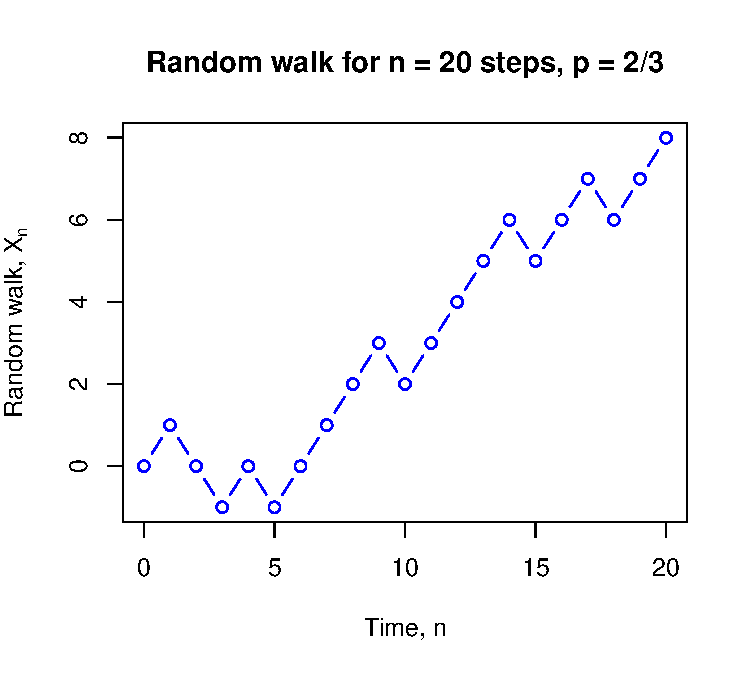
\includegraphics[width=0.5\linewidth]{math2750_files/figure-latex/rw-pics-1} 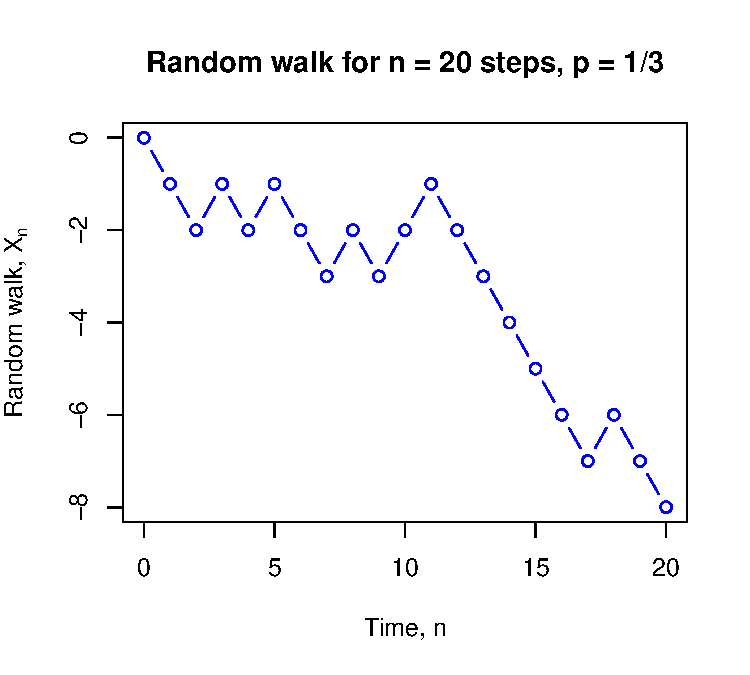
\includegraphics[width=0.5\linewidth]{math2750_files/figure-latex/rw-pics-2} \caption{Two simulations of random walks.}\label{fig:rw-pics}
\end{figure}

We can write this as a stochastic process \((X_n)\) with discrete time \(n = \{0,1,2,\dots\} = \mathbb Z_+\) and discrete state space \(\mathcal S = \mathbb Z\), where \(X_0 = 0\) and, for \(n \geq 0\), we have
\[ X_{n+1} = \begin{cases} X_n + 1 & \text{with probability $p$,} \\
                             X_n - 1 & \text{with probability $q$.} \end{cases} \]

It's clear from this definition that \(X_{n+1}\) (the future) depends on \(X_n\) (the present), but, given \(X_n\), does not depend on \(X_{n-1}, \dots, X_1, X_0\) (the past). Thus the Markov property holds, and the simple random walk is a \textbf{discrete time Markov process} or \textbf{Markov chain}.

\begin{example}
\protect\hypertarget{exm:rw1}{}\label{exm:rw1}

\emph{What is the probability that after two steps a simple random walk has reached \(X_2 = 2\)?}

To achieve this, the walk must go upwards in both time steps, so \(\mathbb P(X_2 = 2) = pp = p^2\).

\end{example}

\begin{example}
\protect\hypertarget{exm:rw2}{}\label{exm:rw2}

\emph{What is the probability that after three steps a simple random walk has reached \(X_3 = -1\)?}

There are three ways to reach \(-1\) after three steps: up--down--down, down--up--down, or down--down--up. So
\[ \mathbb P(X_3 = -1) = pqq+qpq+qqp = 3pq^2 . \]

\end{example}

\hypertarget{general-random-walks}{%
\subsection{General random walks}\label{general-random-walks}}

An alternative way to write the simple random walk is to put
\begin{equation}
    X_n = X_0 + \sum_{i=1}^n Z_i ,  \label{eq:rw}
  \end{equation}
where the starting point is \(X_0 = 0\) and the \textbf{increments} \(Z_1, Z_2, \dots\) are independent and identically distributed (IID) random variables with distribution given by \(\mathbb P(Z_i = 1) = p\) and \(\mathbb P(Z_i = -1) = q\). You can check that \eqref{eq:rw} means that \(X_{n+1} = X_n + Z_{n+1}\), and that this property defines the simple random walk.

Any stochastic process with the form \eqref{eq:rw} for some \(X_0\) and some distribution for the IID \(Z_i\)s is called a \textbf{random walk} (without the word ``simple'').

Random walks often have state space \(\mathcal S = \mathbb Z\), like the simple random walk, but they could be defined on other state spaces. We could look at higher dimensional simple random walks: in \(\mathbb Z^2\), for example, we could step up, down, left or right each with probability \(\frac14\). We could even have a continuous state space like \(\mathbb R\), if, for example, the \(Z_i\)s had a normal distribution.

We can use this structure to calculate the expectation or variance of any random walk (including the simple random walk).

Let's start with the expectation. For a random walk \((X_n)\) we have
\[ \mathbb E X_n = \mathbb E \left(X_0 + \sum_{i=1}^n Z_i\right) = \mathbb E X_0 + \sum_{i=1}^n \mathbb E Z_i = \mathbb EX_0 + n \mathbb E Z_1 , \]
where we've used the linearity of expectation, and that the \(Z_i\)s are identically distributed.

In the case of the simple random walk, we have \(\mathbb E X_0 = 0\), since we start from \(0\) with certainty, and
\[ \mathbb E Z_1 = \sum_{z \in \mathbb Z} z \mathbb P(Z_1 = z) = 1\times p + (-1)\times q = p-q .\]
Hence, for the simple random walk, \(\mathbb EX_n = n(p-q)\).

If \(p > \frac12\), then \(p > q\), so \(\mathbb E X_n\) grows ever bigger over time, while if \(p < \frac12\), then \(\mathbb E X_n\) grows ever smaller (that is, negative with larger absolute value) over time. If \(p = \frac12 = q\), which is the case of the simple symmetric random walk, then then the expectation \(\mathbb E X_n = 0\) is zero for all time.

Now the variance of a random walk. We have
\[ \operatorname{Var}(X_n) = \operatorname{Var}\left(X_0 + \sum_{i=1}^n Z_i\right) = \operatorname{Var}X_0 + \sum_{i=1}^n \operatorname{Var}Z_i = \operatorname{Var}X_0 + n \operatorname{Var}Z_1 , \]
where it was crucial that \(X_0\) and all the \(Z_i\)s were independent (so we had no covariance terms).

For the simple random walk we have \(\operatorname{Var}X_0 = 0\), since we always start from \(0\) with certainty. To calculate the variance of the increments, we write
\begin{align*}
  \operatorname{Var}(Z_1) &= \mathbb E (Z_1 - \mathbb EZ_1)^2 \\
            &= p\big(1 - (p-q)\big)^2 + q \big( {-1} - (p-q)\big)^2\\
            &= p(2q)^2 + q(-2p)^2\\
            &= 4pq^2 + 4p^2q \\
            &= 4pq(p+q) \\
            &= 4pq .
  \end{align*}
Here we've used that \(1-p = q\), \(1-q=p\), and \(p+q = 1\); you should take a few moments to check you've followed the algebra here. Hence the variance of the simple random walk is \(4pqn\). We see that (unless \(p\) is \(0\) or \(1\)) the variance grows over time, so it becomes harder and harder to predict where the random walk will be.

The variance of the simple symmetric random walk is \(4 \frac12 \frac12 n = n\).

For large \(n\), we can use a normal approximation for a random walk. Suppose the increments process \((Z_n)\) has mean \(\mu\) and variance \(\sigma^2\), and that the walk starts from \(X_0 = 0\). Then we have \(\mathbb E X_n = \mu n\) and \(\operatorname{Var}(X_n) = \sigma^2 n\), so for large \(n\) we can use the normal approximation \(X_n \approx \mathrm{N}(\mu n, \sigma^2 n)\). (Remember, of course, that the \(X_n\) are not independent.) To be more formal, the central limit theorem tells us that, as \(n \to \infty\), we have
\[ \frac{X_n - n\mu}{\sigma \sqrt{n}} \to \mathrm{N}(0,1) . \]

\hypertarget{exact-distribution}{%
\subsection{Exact distribution of the simple random walk}\label{exact-distribution}}

We have calculated the expectation and variance of any random walk. But for the simple random walk, we can in fact give the exact distribution, by writing down an exact formula for \(\mathbb P(X_n = i)\) for any time \(n\) and any state \(i\).

Recall that, at each of the first \(n\) times, we independently take an upward step with probability \(p\), and otherwise take a downward step. So if we let \(Y_n\) be the number of upward steps over the first \(n\) time periods, we see that \(Y_n\) has a binomial distribution \(Y_n \sim \text{Bin}(n,p)\).

Recall that the binomial distribution has probability
\[  \mathbb P(Y_n = k)  = \binom nk p^k (1-p)^{n-k} = \binom nk p^k q^{n-k} , \]
for \(k = 0,1,\dots, n\), where \(\binom{n}{k}\) is the binomial coefficient ``\(n\) choose \(k\)''.

If \(Y_n = k\), that means we've taken \(k\) upward steps and \(n-k\) downward steps, leaving us at position \(k - (n-k) = 2k - n\). Thus we have that
\begin{equation}
  \mathbb P(X_n = 2k - n) = \mathbb P(Y_n = k) = \binom nk p^k q^{n-k} .  \label{eq:bin}
  \end{equation}

Note that after an odd number of time steps \(n\) we're always at an odd-numbered state, since \(2k - \text{odd} = \text{odd}\), while after an even number of time steps \(n\) we're always at an even-numbered state, since \(2k - \text{even} = \text{even}\).

Writing \(i = 2k - n\) gives \(k = (n+i)/2\) and \(n-k = (n-i)/2\). So we can rearrange \eqref{eq:bin} to see that the distribution for the simple random walk is
\[ \mathbb P(X_n = i) =  \binom{n}{(n+i)/2} p^{(n+i)/2} q^{(n-i)/2} , \]
when \(n\) and \(i\) have the same parity with \(-n \leq i \leq n\), and is \(0\) otherwise.

In the special case of the simple symmetric random walk, we have
\[ \mathbb P(X_n = i) = \binom{n}{(n+i)/2} \left(\frac12\right)^{(n+i)/2} \left(\frac12\right)^{(n-i)/2} = \binom{n}{(n+i)/2} 2^{-n} . \]

\textbf{In the next section}, we look at a gambling problem based on the simple random walk.

\hypertarget{P01}{%
\section*{Problem Sheet 1}\label{P01}}
\addcontentsline{toc}{section}{Problem Sheet 1}

\commtrue

You should attempt all these questions and write up your solutions in advance of your workshop in week 2 (Monday 1 or Tuesday 2 February) where the answers will be discussed.

\textbf{1.} When designing a model for a quantity that changes over time, one has many decisions to make:

\begin{itemize}
\tightlist
\item
  Discrete or continuous state space?
\item
  Discrete or continuous index set for time?
\item
  Deterministic or stochastic model?
\item
  If a stochastic model is chosen, is it reasonable to assume that the Markov property holds?
\end{itemize}

What would you decide for the following scenarios:

\textbf{(a)} The percentage of UK voters with a positive opinion of Boris Johnson in a weekly tracking poll.

\textbf{(b)} The number of points won by a football league club throughout the season.

\textbf{(c)} The temperature of a bowl of water placed in an oven.

\textbf{(d)} The number of people inside the University of Leeds library.

\begin{myanswers}

\emph{Suggestions.} This question is meant to inspire discussion, so there are not necessarily right and wrong answers. If I were designing the models, however, my choices might be these:

\textbf{(a)} Discrete space if percentages are given to nearest 1\%, otherwise continuous; discrete time (weekly); stochastic; the Markov property might be appropriate, perhaps using some sort of random walk.

\textbf{(b)} Discrete space (number of points); discrete time (update after each game); stochastic; the Markov property might be appropriate, depending on if you think teams can have non-Markovian ``winning streaks'' (or losing streaks) that don't reflect underlying performance.

\textbf{(c)} Continuous space (temperature); continuous time; if the oven is reliable and the experiment carried out carefully, a deterministic model might be sufficient.

\textbf{(d)} Discrete space (number of people); continuous time; stochastic; Markov property might not be appropriate due to `bursts' of people leaving during fire drills or entering when it starts raining.

\end{myanswers}

\textbf{2.} A fair six-sided dice is rolled twice, resulting in the
values \(X_1, X_2 \in \{1, 2, \ldots, 6\}\). Let \(Y = X_1 + X_2\) be the total score.
Calculate:

\textbf{(a)} the probability \(\mathbb P(Y = 10)\);

\begin{myanswers}

\emph{Solution.} The following table illustrates the possible outcomes \(Y\) of the experiment. Each cell of the table is an equally probable outcome.

\begin{center}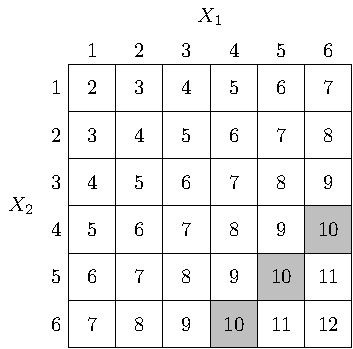
\includegraphics{math2750_files/figure-latex/dice-1} \end{center}

There are 3 possible ways to get \(Y=10\) (the grey cells in the table) out of the \(36\) possible outcomes, so we have \(\mathbb P(Y = 10) = 3/36 = 1/12\).

\end{myanswers}

\textbf{(b)} the conditional probability \(\mathbb P(Y=10 \mid X_1=x)\) for \(x=1, 2, \ldots, 6\);

\begin{myanswers}

\emph{Solution.} Conditioning on \(X_1 = x\) means restricting our attention only to column \(x\) of the table. Each column has \(6\) equally probably cells. For \(x=1,2,3\), none of the entries equal \(10\), so \(\mathbb P(Y=10 \mid X_1=x) = 0/6 = 0\). For each of \(x=4,5,6\), one of the entries equals \(10\), so \(\mathbb P(Y=10 \mid X_1=x) = 1/6\).

\end{myanswers}

\textbf{(c)} the conditional probability \(\mathbb P(X_1=x \mid Y=10)\) for \(x=1, 2, \ldots, 6\).

\begin{myanswers}

\emph{Solution.} Conditioning on \(Y =10\) means restricting our attention only to the \(3\) shaded cells, which are each equally likely. For \(x=1,2,3\), none of the shaded cells are in column \(x\), so \(\mathbb P(X_1=x \mid Y=10) = 0/3 = 0\). For each of \(x=4,5,6\), one of the shaded cells is in column \(x\), so \(\mathbb P(X_1=x \mid Y=10) = 1/3\).

\end{myanswers}

\textbf{3.} Let \((X_n)\) be a simple random walk starting from \(X_0 = 0\) and that at each step goes up one with probability \(p\) or down one with probability \(q = 1-p\). What are:

\textbf{(a)} \(\mathbb P(X_5 = 3)\),

\begin{myanswers}

\emph{Solution.} To get \(X_5 = 3\), we must take \(4\) steps up and \(1\) step down. The down step can be at any of the \(5\) time steps. Therefore we have \(\mathbb P(X_5 = 3) = 5p^4q\).

\end{myanswers}

\textbf{(b)} \(\mathbb P(X_5 = 3 \mid X_2 = 2)\),

\begin{myanswers}

\emph{Solution.} Once we're at \(X_2 = 2\), we must take \(2\) steps up and \(1\) step down over the next \(3\) time steps. So \(\mathbb P(X_5 = 3 \mid X_2 = 2) = 3p^2q\).

\end{myanswers}

\textbf{(c)} \(\mathbb P(X_n = n-2)\),

\begin{myanswers}

\emph{Solution.} This requires \(n-1\) steps up and \(1\) step down, and the down step can be at any of the \(n\) time steps. So \(\mathbb P(X_n = n-2) = np^{n-1}q\).

\end{myanswers}

\textbf{(d)} \(\mathbb E X_4\),

\begin{myanswers}

\emph{Solution.} The increments \(Z_n = X_n - X_{n-1}\) have expectation \(1p + (-1)q = p - q\), so \(\mathbb E X_4 = 4(p-q)\).

\end{myanswers}

\textbf{(e)} \(\mathbb E(X_6 \mid X_4 = 2)\),

\begin{myanswers}

\emph{Solution.} We are already at 2, then another two increments will take us up \(2(p-q)\) on average. Therefore \(\mathbb E(X_6 \mid X_4 = 2) = 2 + 2(p-q)\).

\end{myanswers}

\textbf{4.} The price \(X_n\) of a stock at the close of day \(n\) is modelled as a Gaussian random walk, where the increments \((Z_n)\) have a normal distribution \(Z_n \sim \text{N}(\mu, \sigma^2)\). The model assumes a drift of \(\mu = 0.7\) and a volatility of \(\sigma = 2.2\). The initial price is \(X_0 = 42.3\).

\textbf{(a)} Calculate the mean and variance of the price of the stock at the close of day \(5\).

\begin{myanswers}

\emph{Solution.} The mean and variance are
\begin{gather*}
  \mathbb EX_5 = \mathbb E X_0 + n \mathbb E Z_1 = 42.3 + 5 \cdot 0.7 = 45.8 , \\
  \operatorname{Var}X_5 = \operatorname{Var}X_0 + n \operatorname{Var}Z_1 = 0 + 5 (2.2)^2 = 24.2 .
  \end{gather*}

\end{myanswers}

\textbf{(b)} Give a 95\% prediction interval for the price at the close of day 5. (You might find it useful to recall that, if \(W \sim \text{N}(0,1)\) is a standard normal random variable, then \(\mathbb P(W \leq 1.96) = 0.975\).)

\begin{myanswers}

\emph{Solution.} Note that \(X_5\) itself is normally distributed, so \(X_5 \sim \text{N}(45.8,24.2)\). The 95\% prediction interval for a normal distribution \(\text{N}(\mu, \sigma^2)\) is \((\mu - 1.96\sigma, \mu + 1.96\sigma)\), so the prediction interval for \(X_5\) is
\[ \big(45.8 - 1.96\sqrt{24.2},  45.8 + 1.96\sqrt{24.2}\big) = (36.16, 55.44) . \]

\end{myanswers}

\textbf{(c)} After day 4, the prices at the end of each of the first four days have been recorded as \(X_1 = 44.4, X_2 = 44.0, X_3 = 47.1, X_4 = 47.8\). Update your prediction interval for the price at the close of day 5, and comment on how it differs from the earlier prediction interval.

\begin{myanswers}

\emph{Solution.} By the Markov property, \(X_5\) depends on \(X_4\), but given \(X_4\) does not depend on the other values, which we can therefore ignore. Since \(X_5 = X_4 + Z_5\), we have
\begin{gather*}
  \mathbb E(X_5 \mid X_4) = X_4 + \mathbb E Z_5 = 47.8 + 0.7 = 48.5 \\
  \operatorname{Var}(X_5 \mid X_4) = 0 + \operatorname{Var}Z_5 = 0 + (2.2)^2 = 4.84.
  \end{gather*}
The desired prediction interval is
\[ \big(48.5 - 1.96\sqrt{4.84},  48.5+ 1.96\sqrt{4.84}\big) = (44.19, 52.81) . \]
Compared to before, the centre of the prediction interval is slightly higher, because the stock has outperformed expectations so far, and the interval is much narrower, because as we get closer to day 5 we become less uncertain.

\end{myanswers}

\textbf{5.} A gambler decides to model her total winnings as a simple random walk starting from \(X_0 = 0\) that at each time goes up one with probability \(p\) and down one with probability \(1-p\), but where \(p\) is unknown. The first \(10\) recordings, \(X_1\) to \(X_{10}\), are
\[ (1, 2, 1, 2, 3, 4, 5, 6, 5, 6) . \]

\textbf{(a)} What would you guess for the value of \(p\), given this data?

\begin{myanswers}

\emph{Solution.} In \(10\) time steps, the process went up \(k = 8\) times and down \(n - k = 2\) times. So it seems reasonable to guess that \(p\) has the value \(\hat p = \frac{8}{10} = 0.8\).

\end{myanswers}

\textbf{(b)} More generally, how would you estimate \(p\) from the data \(X_0 = 0, X_1 = x_1, X_2 = x_2, \dots, X_n = x_n\)?

\begin{myanswers}

\emph{Solution.} We will estimate \(\hat p = k/n\), where \(k\) is the number of upward steps. We saw in lectures that \(k = (n + x_n)/2\), so our estimate is
\[ \hat p = \frac{n + x_n}{2n} = \frac12\ + \frac{x_n}{2n} . \]

\end{myanswers}

\textbf{(c)} Show that your estimate is in fact the maximum likelihood estimate of \(p\).

\begin{myanswers}

\emph{Solution.} The concept of ``maximum likelihood estimation'' will be known to those who have done MATH2715; this might be new for those who didn't take that course.

Let \(k = (n + x_n)/2\) be the number of upward steps. Then the ``likelihood'' is the probability mass function
\[ f(\mathbf x; p) = p^{k}(1-p)^{n-k} , \]
since we take \(k\) steps up and \(n-k\) steps down.
Given \(\mathbf x\) (or equivalently \(k\)) the ``maximum likelihood estimate'' is the value of \(p\) that maximises this likelihood.

As is often the case, it's equivalent but actually more convenient to maximise the log-likelihood
\[ \ell(\mathbf x; p) = \ln f(\mathbf x; p) = k \ln p + (n-k)\ln(1-p) .\]
We can perform the maximisation by differentiating and setting equal to \(0\). The derivative is
\[ \frac{\text{d}}{\text{d}p} \ell(\mathbf x; p) = \frac kp - \frac{n-k}{1-p} ,\]
so the maximum likelihood estimate \(\hat p\) satisfies
\[ 0 = \frac k{\hat p} - \frac{n-k}{1-\hat p} . \]

Solving this by clearing denominators we get
\[ 0 = (k - k\hat p) - (n\hat p - k\hat p) = k - n \hat p , \]
and rearranging gives \(\hat p = k/n\) as desired.

\end{myanswers}

\hypertarget{S03-gamblers-ruin}{%
\section{Gambler's ruin}\label{S03-gamblers-ruin}}

\begin{itemize}
\tightlist
\item
  The gambler's ruin Markov chain
\item
  Equations for probability of ruin and expected duration of the game by conditioning on the first step
\end{itemize}

\hypertarget{ruin-chain}{%
\subsection{Gambler's ruin Markov chain}\label{ruin-chain}}

Consider the following gambling problem. Alice is gambling against Bob. Alice starts with £\(a\) and Bob starts with £\(b\). It will be convenient to write \(m = a + b\) for the total amount of money, so Bob starts with £\((m-a)\). At each step of the game, both players bet £1; Alice wins £1 off Bob with probability \(p\), or Bob wins £1 off Alice with probability \(q\). The game continues until one player is out of money (or is ``ruined'').

Let \(X_n\) denote how much money Alice has after \(n\) steps of the game. We can write this as a stochastic process with discrete time \(n \in \{0,1,2,\dots\} = \mathbb Z_+\) and discrete state space \(\mathcal S = \{0,1,\dots,m\}\). Then \(X_0 = a\), and, for \(n \geq 0\), we have
\[ X_{n+1} = \begin{cases} X_n + 1 & \text{with probability $p$ if $1\leq X_n \leq m-1$,} \\
                           X_n - 1 & \text{with probability $q$ if $1\leq X_n \leq m-1$,} \\
                           0       & \text{if $X_n = 0$,} \\
                           m       & \text{if $X_n = m$.} \end{cases} \]
So Alice's money goes up one with probability \(p\) or down one with probability \(q\), unless the game is already over with \(X_n = 0\) (Alice is ruined) or \(X_n = m\) (Alice has won all Bob's money, so Bob in ruined).

We see that the gambler's ruin process \((X_n)\) clearly satisfies the Markov property: the next step \(X_{n+1}\) depends on where we are now \(X_n\), but, given that, does not depend on how we got here.

The gambler's ruin process is exactly like a simple random walk started from \(X_0 = a\) except that we have \textbf{absorbing barriers} and \(0\) and \(m\), where the random walk stops because one of the players has ruined. (One could also consider random walks with \textbf{reflecting barriers}, that bounce the random walk back into the state space, or \textbf{mixed barriers} that are absorbing or reflecting at random.)

There are two questions about the gambler's ruin that we'll try to answer in this section:

\begin{enumerate}
\def\labelenumi{\arabic{enumi}.}
\tightlist
\item
  What is the probability that the game ends by Alice ruining?
\item
  How long does the game last on average?
\end{enumerate}

\hypertarget{ruin-probability}{%
\subsection{Probability of ruin}\label{ruin-probability}}

The gambling game continues until either Alice is ruined (\(X_n = 0\)) or Bob is ruined (\(X_n = m\)). A natural question to ask is: What is the probability that the game ends in Alice's ruin?

Let us write \(r_i\) for the probability Alice ends up ruined if she currently has £\(i\). Then the probability of ruin for the whole game is \(r_a\), since Alice initially starts with £\(a\). The probability Bob will end up ruined is \(1 - r_a\), since one of the players must lose.

What can we say about \(r_i\)? Clearly we have \(r_0 = 1\), since \(X_n = 0\) means that Alice has run out of money and is ruined, and \(r_m = 0\), since \(X_n = m\) means that Alice has won all the money and Bob is ruined. What about when \(1 \leq i \leq m-1\)?

The key is to \emph{condition on the first step}. That is, we can write
\begin{align*}
\mathbb P(\text{ruin}) &= \mathbb P(\text{win first round}) \, \mathbb P(\text{ruin} \mid \text{win first round}) \\
&\qquad{}\quad {}+ \mathbb P(\text{lose first round}) \, \mathbb P(\text{ruin} \mid \text{lose first round}) \\
&= p\,\mathbb P(\text{ruin} \mid \text{win first round}) + q \,\mathbb P(\text{ruin} \mid \text{lose first round}) .
\end{align*}
Here we have conditioned on whether Alice wins or loses the first round. More formally, we have used the \textbf{law of total probability}, which says that if the events \(B_1, \dots, B_k\) are disjoint and cover the whole sample space, then
\[ \mathbb P(A) = \sum_{i=1}^k \mathbb P(B_i) \, \mathbb P(A \mid B_i) . \]
Here, \(\{\text{Alice wins the first round}\}\) and \(\{\text{Alice loses the first round}\}\) are indeed disjoint events that cover the whole sample space. This idea of ``conditioning on the first step'' will be the most crucial tool throughout this whole module.

If Alice wins the first round from having £\(i\), she now has £\((i+1)\). Her probability of ruin is now \(r_{i+1}\), because, by the Markov property, it's as if the game were starting again with Alice having £\((i+1)\) to start with. The Markov property tells us that it doesn't matter \emph{how} Alice got to having £\((i+1)\), it only matters how much she has now. Similarly, if Alice loses the first round, she now has £\((i-1)\), and the ruin probability is \(r_{i-1}\). Hence we have
\[ r_i = pr_{i+1} + qr_{i-1}. \]

Rearranging, and including the ``boundary conditions'', we see that the equation we want to solve is
\[ pr_{i+1} - r_i + qr_{i-1} = 0 \qquad \text{subject to} \qquad r_0 = 1,\ r_m = 0. \]
This is a \textbf{linear difference equation} -- and, because the left-hand side is \(0\), we call it a \textbf{homogeneous} linear difference equation.

We will see how to solve this equation in the next lecture. We will see that, if we set \(\rho = q/p\), then the ruin probability is given by
\[ r_a = \begin{cases} \displaystyle\frac{\rho^a - \rho^m}{1 - \rho^m} & \text{if $\rho \neq 1$,} \\[0.35cm]
           1 - \displaystyle\frac{a}{m} & \text{if $\rho = 1$.} \end{cases} \]
Note that \(\rho = 1\) is the same as the symmetric condition \(p = q = \frac12\).

Imagine Alice is not playing against a similar opponent Bob, but rather is up against a large casino. In this case, the casino's capital £\((m-a)\) is typically much bigger than Alice's £\(a\). We can model this by keeping \(a\) fixed taking a limit \(m \to \infty\). Typically, the casino has an ``edge'', meaning they have a better than \(50:50\) chance of winning; this means that \(q > p\), so \(\rho > 1\). In this case, we see that the ruin probability is
\[ \lim_{m \to \infty} r_a = \lim_{m \to \infty} \frac{\rho^a - \rho^m}{1 - \rho^m} = \lim_{m \to \infty} \frac{\rho^a/\rho^m - 1}{1/\rho^m - 1} = \frac{0-1}{0-1} = 1, \]
so Alice will be ruined with certainty.

Even with a generous casino that offered an exactly fair game with \(p = q = \frac12\), so \(\rho = 1\), we would have
\[ \lim_{m \to \infty} r_a = \lim_{m \to \infty}\left( 1 - \frac{a}{m} \right) = 1-0 = 1 , \]
so, even with this fair game, Alice would still be ruined with certainty.

(The official advice of the University of Leeds module MATH2750 is that you shouldn't gamble against a casino if you can't afford to lose.)

\hypertarget{expected-duration}{%
\subsection{Expected duration of the game}\label{expected-duration}}

We could also ask for how long we expect the game to last.

We approach this like before. Let \(d_i\) be the expected duration of the game from a point when Alice has £\(i\). Our boundary conditions are \(d_0 = d_m = 0\), because \(X_n = 0\) or \(X_n = m\) means that the game is over with Alice or Bob ruined. Again, we proceed by conditioning on the first step, so
\begin{align*}
\mathbb E(\text{duration}) &= \mathbb P(\text{win first round}) \, \mathbb E(\text{duration} \mid \text{win first round}) \\
&\qquad{}+ \mathbb P(\text{lose first round}) \, \mathbb E(\text{duration} \mid \text{lose first round}) \\
&= p\,\mathbb E(\text{duration} \mid \text{win first round}) + q \,\mathbb E(\text{duration} \mid \text{lose first round}) .
\end{align*}
More formally, we've used another version of the law of total probability,
\[ \mathbb E(X) = \sum_{i=1}^k \mathbb P(B_i) \, \mathbb E(X \mid B_i) , \]
or, alternatively, the \textbf{tower law} for expectations
\[ \mathbb E(X) = \mathbb E_Y \mathbb E (X \mid Y) = \sum_{y} \mathbb P(Y= y)\, E(X \mid Y = y), \]
where, in our case, \(Y\) was the outcome of the first round.

Now, the expected duration given we win the first round is \(1 + d_{i+1}\). This is because the round itself takes \(1\) time step, and then, by the Markov property, it's as if we are starting again from \(i+1\). Similarly, the expected duration given we lose the first round is \(1 + d_{i-1}\). Thus we have
\[ d_i = p(1 + d_{i+1}) + q (1 + d_{i-1}) = 1 + pd_{i+1} + qd_{i-1} . \]
Don't forget the 1 that counts the current round!

Rearranging, and including the boundary conditions, we have another linear difference equation:
\[ pd_{i+1} - d_i + qd_{i-1} = -1 \qquad \text{subject to} \qquad d_0 = 0,\ d_m = 0. \]
Because the right-hand side, \(-1\), is nonzero, we call this an \textbf{inhomogeneous} linear difference equation.

Again, we'll see how to solve this in the next lecture, and will find that the solution is given by
\[ d_a = \begin{cases} {\displaystyle \frac{1}{q-p} \left(a - m\frac{1-\rho^a}{1- \rho^m} \right)} & \text{if $\rho \neq 1$,} \\
\displaystyle a(m-a) & \text{if $\rho = 1$.} \end{cases} \]

Thinking again of playing against the casino, with \(q > p\), \(\rho > 1\), and \(m \to \infty\), we see that the expected duration is
\[ \lim_{m\to\infty} d_a = \lim_{m\to\infty} \frac{1}{q-p} \left(a - m\frac{1-\rho^a}{1 - \rho^m} \right)  = \frac{1}{q-p} \left(a - 0 \right) = \frac{a}{q-p} , \]
since \(\rho^m\) grows much quicker than \(m\). So Alice ruins with certainty, and it will take time \(a/(q-p)\), on average.

In the case of the generous casino, though, with \(q = p\), so \(\rho = 1\), we have
\[ \lim_{m\to\infty} d_a =  \lim_{m\to\infty} a(m-a) = \infty .  \]
So here, Alice will ruin with certainty, but it may take a very long time until the ruin occurs, since the expected duration is infinite.

\textbf{In the next section}, we see how to solve linear difference equations, in order to find the ruin probability and expected duration of the gambler's ruin.

\hypertarget{S04-ldes}{%
\section{Linear difference equations}\label{S04-ldes}}

\begin{itemize}
\tightlist
\item
  How to solve homogeneous and inhomogeneous linear difference equations
\item
  Solving for probability of ruin and expected duration of the gambler's ruin
\end{itemize}

In \protect\hyperlink{S03-gamblers-ruin}{the previous section}, we looked at the probability of ruin and expected duration of the gambler's ruin process. We set up linear difference equations to find these. In this section, we'll learn how to solve these equations.

A \textbf{linear difference equation} is an equation that looks like
\begin{equation}
a_k x_{n+k} + a_{k-1} x_{n+k-1} + \cdots + a_1 x_{n+1} + a_0 x_n = f(n) \label{eq:lde} 
\end{equation}
for \(n = 0,1,\dots\), where the \(a_i\) are given constants, \(f(n)\) is a given function, and we want to solve for the sequence \((x_n)\). The equation normally comes with some extra conditions, such as the value of the first few \(x_n\)s.

When the right-hand side of \eqref{eq:lde} is zero, so \(f(n) = 0\), we say the equation is \textbf{homogeneous}; when the right-hand side is nonzero, it is \textbf{inhomogeneous}. The number \(k\), where there are \(k+1\) terms on the left-hand side, is called the \textbf{degree} of the equation; we are mostly interested in second-degree linear difference equations, which have three terms on the left-hand side.

\hypertarget{hom-ldes}{%
\subsection{Homogeneous linear difference equations}\label{hom-ldes}}

We start with the homogeneous case, which is simpler.

Consider a homogeneous linear difference equation. We shall use the second-degree example
\[ x_{n+2} - 5x_{n+1} + 6x_{n} = 0 \qquad \text{subject to } x_0 = 4, x_1 = 9 .  \]
Here, the conditions on \(x_0\) and \(x_1\) are \textbf{initial conditions}, because they tell us how the sequence \((x_n)\) starts.

For the moment, we shall put the initial conditions to the side and just worry about the equation
\[ x_{n+2} - 5x_{n+1} + 6x_{n} = 0 . \]
We start by guessing there might be a solution of the form \(x_n = \lambda^n\) for some constant \(\lambda\). We can find out if there is such a solution by substituting in \(x_n = \lambda^n\), and seeing if there's a \(\lambda\) that solves the equation. For our example, we get
\[ \lambda^{n+2} - 5 \lambda^{n+1} + 6\lambda^n = 0 . \]
After cancelling off a common factor of \(\lambda^n\), we get
\[ \lambda^2 - 5 \lambda + 6 = 0 . \]
This is called the \textbf{characteristic equation}. For a general homogeneous linear difference equation \eqref{eq:lde}, the characteristic equation is
\begin{equation}
  a_k \lambda^{k} + a_{k-1} \lambda^{k-1} + \cdots + a_1 \lambda + a_0 = 0 .  \label{eq:cheq} 
\end{equation}
When writing out answers to questions, you can jump straight to the characteristic equation.

We can now solve the characteristic equation for \(\lambda\). In our example, we can factor the left-hand side to get \((\lambda - 3)(\lambda - 2) = 0\), which has solutions \(\lambda = 2\) and \(\lambda = 3\). Thus \(x_n = 2^n\) and \(x_n = 3^n\) both solve our equation. In fact, since the right-hand side of the equation is \(0\), any linear combination of these two solutions is a solution also, thus we get the \textbf{general solution}
\[ x_n = A 2^n + B 3^n , \]
which is a solution for any values of the constants \(A\) and \(B\).

For a general characteristic equation with distinct roots \(\lambda_1, \lambda_2, \dots, \lambda_k\), the general solution is
\[ x_n = C_1 \lambda_1^n + C_2 \lambda_2^n + \cdots + C_k \lambda_k^n . \]
If we have a repeated root -- say, \(\lambda_1 = \lambda_2 = \cdots = \lambda_r\) is repeated \(r\) times -- than you can check that a solution is given by
\[ x_n = (D_0 + D_1 n + \cdots + D_{r-1} n^{r-1}) \lambda_1^n , \]
which should take its place in the general solution.

Once we have the general solution, we can use the extra conditions to find the values of the constants. In our example, we can use the initial conditions to find out the values of \(A\) and \(B\). We see that
\begin{gather*}
x_0 = A2^0 + B3^0 = A + B = 4 , \\
x_1 = A2^1 + B3^1 = 2A + 3B = 9 .
\end{gather*}
We can now solve this pair of simultaneous equations to solve for \(A\) and \(B\). By subtracting twice the first equation from the second we get \(B = 1\), and substituting this into the first equation we get \(A = 3\). Thus the solution is
\[ x_n = 3\cdot 2^n + 3^n . \]

In conclusion, the process here was:

\begin{enumerate}
\def\labelenumi{\arabic{enumi}.}
\tightlist
\item
  Find the general solution by writing down and solving the characteristic equation.
\item
  Use the extra conditions to find the values of the constants in the general solution.
\end{enumerate}

Here are two more examples. These also give an idea of how I would expect you to set out your own answers to similar problems.

\begin{example}
\protect\hypertarget{exm:lde1}{}\label{exm:lde1}

\emph{Solve the homogeneous linear difference equation}
\[ x_{n+2} - x_{n+1} - 6x_n = 0 \qquad \text{subject to} \quad x_0 = 3,\quad x_1 = 4 . \]

\emph{Step 1.} The characteristic equation is
\[ \lambda^2 - \lambda - 6 = 0 . \]
We can solve this by factorising it as \((\lambda - 3) (\lambda + 2) = 0\),
to find the solutions \(\lambda_1 = -2\) and \(\lambda_2 = 3\). Thus the general solution is
\[ x_n = A(-2)^n + B3^n . \]

\emph{Step 2.} Substituting the initial conditions into the general solution, we have
\begin{align*}
x_0 &= A(-2)^0 + B3^0 = A + B = 3 \\
x_1 &= A(-2)^1 + B3^1 = -2A + 3B = 4 .
\end{align*}
We can add twice the first equation to the second to get \(5B = 10\), so \(B=2\). We can substitute this into the first equation to get \(A = 1\).

The solution is therefore
\[ x_n = 1\cdot(-2)^n + 2 \cdot 3^n = (-2)^n + 2 \cdot 3^n . \]

\end{example}

\begin{example}
\protect\hypertarget{exm:lde2}{}\label{exm:lde2}

\emph{Solve the homogeneous linear difference equation}
\[ x_{n+2} + 4x_{n+1} +4x_n = 0 \qquad \text{subject to} \quad x_0 = 2,\quad x_1 = -6 . \]

\emph{Step 1.} The characteristic equation is
\[ \lambda^2 + 4\lambda + 4 = 0 . \]
We can solve this by factorising it as \((\lambda + 2)^2 = 0\), to find a repeated root \(\lambda_1 = \lambda_2 = -2\). Thus the general solution is
\[ x_n = (A + Bn) (-2)^n . \]

\emph{Step 2.} Substituting the initial conditions into the general solution, we have
\begin{align*}
x_0 &= (A + B0)(-2)^0 = A = 2 \\
x_1 &= (A + B1)(-2)^1 = -2A - 2B = -6 .
\end{align*}
The first immediately gives \(A = 2\), and substituting this into the second equation gives \(B = 1\).

The solution is therefore
\[ x_n = (2 + n)(-2)^n . \]

\end{example}

\hypertarget{ruin-probability-solve}{%
\subsection{Probability of ruin for the gambler's ruin}\label{ruin-probability-solve}}

In the last lecture we saw that probability of ruin for the gambler's ruin process is the solution to
\[ pr_{i+1} - r_i + qr_{i-1} = 0 \qquad \text{subject to} \qquad r_0 = 1,\ r_m = 0 , \]
where the extra conditions here are \textbf{boundary conditions}, because they tell us what happens at the boundaries of the state space.

The characteristic equation is
\[ p\lambda^2 - \lambda + q = 0 .\]
We can solve the characteristic equation by factorising it as \((p \lambda - q)(\lambda - 1) = 0\). (It might take a moment to check this really is a factorisation of the characteristic equation. Hint: we've used that \(p+q=1\).) So the characteristic equation has roots \(\lambda = q/p\), which we called \(\rho\) last time, and \(\lambda = 1\). Now, if \(\rho = 1\) (so \(p = q = \frac12\)) we have a repeated root, while if \(\rho \neq 1\) we have distinct roots, so we'll need to deal with the two cases separately.

First, the case \(\rho \neq 1\). Since the two roots are distinct, we have the general solution
\[ r_i = A\rho^i + B1^i = A\rho^i + B . \]

We can now use the boundary conditions to find \(A\) and \(B\). We have
\begin{gather*} r_0 = A \rho^0 + B = A+B = 1, \\
                r_m = A \rho^m + B = 0 . \end{gather*}
From the first we get \(B = 1-A\), which we substitute into the second to get
\[ A\rho^m + 1 - A = 0 \quad \Rightarrow \quad A = \frac{1}{1-\rho^m} , \]
and hence
\[ B = 1 - A = 1 - \frac{1}{1-\rho^m} = - \frac{\rho^m}{1 - \rho^m} . \]
Thus the solution is
\[ r_i = \frac{1}{1-\rho^m} \rho^i -  \frac{\rho^m}{1 - \rho^m} = \frac{\rho^i - \rho^m}{1 - \rho^m}  , \]
as we claimed last time.

Second, the case \(\rho = 1\). Now we have a repeated root \(\lambda = 1\), so the general solution is
\[ r_i = (A + Bi) 1^i = A+Bi . \]

Again, we use the boundary conditions, to get
\begin{gather*} r_0 = A + B\cdot 0 = A = 1, \\
r_m = A + Bm = 0 , \end{gather*}
and we immediately see that \(A = 1\) and \(B = -1/m\). Thus the solution is
\[ r_i = 1 - \frac{1}{m}i = 1 - \frac{i}{m} , \]
as claimed last time.

\hypertarget{inhom-ldes}{%
\subsection{Inhomogeneous linear difference equations}\label{inhom-ldes}}

Solving inhomogeneous linear difference equations requires three steps:

\begin{enumerate}
\def\labelenumi{\arabic{enumi}.}
\tightlist
\item
  Find the general solution to the \emph{homogeneous} equation by writing down and solving the characteristic equation.
\item
  By making an ``educated guess'', find a solution (a ``particular solution'') to the inhomogeneous equation. The general solution to the inhomogeneous equation is a particular solution plus the general solution to the homogeneous equation.
\item
  Use the extra conditions to find the values of the constants in the general solution.
\end{enumerate}

This idea works because, once you have a particular solution, adding a solution to the \emph{homogeneous} equation to the left-hand side adds zero to the right-hand side, so maintains a solution to the inhomogeneous equation.

Let's work through the example
\[ x_{n+2} - 5x_{n+1} + 6x_{n} = 2 \qquad \text{subject to } x_0 = 4, x_1 = 9 . \]

We already know from earlier that the general solution to the homogeneous equation \(x_{n+2} - 5x_{n+1} + 6x_{n} = 0\) (with a zero on the right-hand side) is
\[ x_n = A2^n + B3^n . \]

We now need to find a \textbf{particular solution} -- that is, any solution -- to our new inhomogeneous equation. The usual process here is to guess a solution with the same ``shape'' as the right-hand side. For example, if the right-hand side is a constant, try a constant for the particular solution. Here our right-hand side is the constant \(2\), so we should try a constant \(x_n = C\). Substituting this into the inhomogeneous equation gives us \(C - 5C + 6C = 2\), thus \(2C = 2\) and \(C = 1\), giving a particular solution \(x_n = 1\). The general solution to the inhomogeneous equation is therefore
\[ x_n = 1 + A2^n + B3^n , \]
the sum of the particular solution \(x_n = 1\) and the general solution to the homogeneous equation.

Because the right-hand side was a constant, we guessed a constant -- this is the main case we will deal with. Other cases you could come across include:

\begin{itemize}
\tightlist
\item
  If the right-hand side is a polynomial of degree \(d\), try a polynomial of degree \(d\).
\item
  If the right-hand side is \(\alpha^n\) for some \(\alpha\), try \(C\alpha^n\).
\item
  If the right-hand side is a constant, but a constant \(C\) doesn't work, try \(Cn\). If that still doesn't work, try \(Cn^2\), and so on. A general rule is that is 1 is a root of the characteristic equation with multiplicity \(m\), you need to try \(Cn^m\). We discuss this case further in the next subsection.
\end{itemize}

Continuing with the example, we use the initial conditions to get the constants \(A\) and \(B\). We have
\begin{gather*}
x_0 = 1 + A2^0 + B3^0 = 1+ A + B = 4 , \\
x_1 = 1 + A2^1 + B3^1 = 1+ 2A + 3B = 9 .
\end{gather*}
The second equation minus twice the first gives \(-1 + B = 1\), so \(B=2\), and substituting that back into the first gives \(A = 1\). Thus the solution is
\[ x_n = 1 + 1\cdot 2^n + 2 \cdot 3^n = 1 + 2^n + 2 \cdot 3^n . \]

Here's another example.

\begin{example}
\protect\hypertarget{exm:lde3}{}\label{exm:lde3}

\emph{Solve the inhomogeneous linear difference equation}
\[ 10 x_{n+2} - 7x_{n+1} + x_n = 8 \qquad \text{subject to} \quad x_0 = 0,\quad x_1 = \tfrac{13}{10} . \]

\emph{Step 1.} The characteristic equation is
\[ 10\lambda^2 - 7\lambda + 1 = 0 . \]
We can solve this by factorising it as
\[ (2\lambda - 1) (5\lambda - 1) = 0 , \]
to find the solutions \(\lambda_1 = \frac12\) and \(\lambda_2 = \frac15\). Thus the general solution of the homogeneous equation is
\[ x_n = A\left(\frac12\right)^n + B\left(\frac15\right)^n . \]

\emph{Step 2.} Since the right hand side of the inhomogeneous equation is a constant, we guess a constant particular solution with shape \(x_n = C\). Substituting in this guess, we get
\[ 10C - 7C + C = 4C = 8 \]
with solution \(C=2\). Thus a particular solution is \(x_n = 2\), and the general solution to the inhomogeneous equation is
\[ x_n = 2 + A\left(\frac12\right)^n + B\left(\frac15\right)^n . \]

\emph{Step 3.} Substituting the initial conditions into the general solution, we have
\begin{align*}
x_0 = 2 + A\left(\frac12\right)^0 + B\left(\frac15\right)^0 = 2 + A + B = 0 \quad &\Rightarrow \quad A + B = -2 \\
x_1 = 2 + A\left(\frac12\right)^1 + B\left(\frac15\right)^1 = 2 + A\frac12 + B\frac15 = \frac{13}{10} \quad &\Rightarrow \quad 5A + 2B = -7.
\end{align*}
We can take twice the first equation abd subtract the second to get \(-3A = 3\), so \(A = -1\). We can substitute this into the second equation to get \(B = -1\).

The solution is therefore
\[ x_n = 2 - \left(\frac12\right)^n - \left(\frac15\right)^n . \]

\end{example}

\hypertarget{duration-solve}{%
\subsection{Expected duration for the gambler's ruin}\label{duration-solve}}

From last time, the expected duration of the gambler's ruin game solves
\[ pd_{i+1} - d_i + qd_{i-1} = -1 \qquad \text{subject to} \qquad d_0 = 0,\ d_m = 0. \]
As before, we divide cases based on whether or not \(\rho = 1\).

First, the case \(\rho \neq 1\). We already know that the general solution to the homogeneous equation is
\[ d_i =  A \rho^i + B . \]

Now we need a particular solution. It's tempting to guess a constant \(C\) for a particular solution, but we know that constants solve the homogeneous equation, since \(d_i = B\) is a solution, so a constant will give right-hand side \(0\), not \(-1\). (We could try out \(x_i = C\) if we wanted; we would get \((p - 1 + q)C = -1\), but \(p-1+q=0\), and \(0 \times C = -1\) has no solution.) The next best try is to go one degree up: let's guess \(x_i = Ci\) instead. This gives
\begin{align*}
  -1 &= pC(i+1) - Ci + qC(i-1)\\
     &= C(pi + p - i + qi - q) \\
     &= C\big((p+q-1)i + (p-q)\big) \\
     &= C(p-q) ,
  \end{align*}
since \(p + q - 1 = 1 - 1 = 0\). This \(C = -1/(p-q) = 1/(q-p)\). Finding a solution for \(C\) shows that our guess worked. The general solution to the inhomogeneous equation is
\[ d_i = \frac{i}{q-p} + A \rho^i + B .  \]

Then to find the constants, we have
\begin{gather*} d_0 = \frac{0}{q-p} + A \rho^0 + B = A+B = 0, \\
                  d_m = \frac{m}{q-p} + A \rho^m + B = 0 , \end{gather*}
which you can check gives
\[ A = -B = \frac{m}{q-p} \cdot \frac{1}{1 - \rho^m} . \]
Hence, the solution is
\[ d_i = \frac{i}{q-p} + \frac{m}{q-p} \frac{1}{1 - \rho^m} \rho^i - \frac{m}{q-p} \frac{1}{1 - \rho^m} =  \frac{1}{q-p} \left(i - m\frac{1-\rho^i}{1- \rho^m} \right) . \]

Second, the case \(\rho = 1\), so \(p = q = \frac12\). We already know that the general solution to the homogeneous equation is
\[ d_i =  A + Bi . \]

We need a particular solution. Since 1 is a double root of the characteristic equation, both constants \(x_i = A\) and linear \(x_i = Bi\) terms solve the homogeneous equation. (You can check that guessing \(x_i = C\) or \(x_i = Ci\) doesn't work, if you like.) So we'll have to go up another degree and try \(x_i = Ci^2\). This gives
\begin{align*}
    -1 &= \tfrac12 C(i+1)^2 - Ci^2 + \tfrac 12 C(i-1)^2 \\
       &= \tfrac12 C(i^2 + 2i + 1 - 2i^2 + i^2 - 2i + 1) \\
       &= \tfrac12 C\big((1-2+1)i^2 + (2-2)i + (1+1)\big) \\
       &=C ,
\end{align*}
so the general solution to the inhomogeneous equation is
\[ d_i = -i^2 + A + Bi .  \]

Then to find the constants, we have
\begin{gather*} d_0 = -0^2 + A + B\cdot0 = A = 0, \\
                  d_m = -m^2 + A + Bm = 0 , \end{gather*}
giving \(A = 0, B = m\). The solution is
\[ d_i = -i^2 + 0 + mi = i(m-i) .\]

\textbf{In the next section}, we move on from the specific cases we've looked at so far to the general theory of discrete time Markov chains.

\hypertarget{P02}{%
\section*{Problem sheet 2}\label{P02}}
\addcontentsline{toc}{section}{Problem sheet 2}

\commfalse

You should attempt all these questions and write up your solutions in advance of your workshop in week 3 (Monday 8 or Tuesday 9 February) where the answers will be discussed.

\textbf{1.} Solve the following linear difference equations:

\textbf{(a)} \(x_{n+2} - 4x_{n+1} + 3x_{n} = 0\), subject to \(x_0 = 0\), \(x_1 = 2\).

\begin{myanswers}

\emph{Solution.} The characteristic equation is \(\lambda^2 - 4\lambda + 3 = 0\), which factorises as \((\lambda - 3)(\lambda - 1) = 0\), with solutions \(\lambda = 1,3\), so the general solution is \(x_n = A1^n + B3^n = A + B3^n\). The initial conditions give \(A+B = 0\) and \(A + 3B = 2\), meaning \(B = 1\) and \(A = -1\). Hence the solution is \(x_n = 3^n - 1\).

\end{myanswers}

\textbf{(b)} \(4x_{n+1} = 4x_n - x_{n-1}\), subject to \(x_0 = 1\), \(x_1 = 0\).

\begin{myanswers}

\emph{Solution.} First, we rearrange to \(4x_{n+1} - 4x_n + x_{n-1} = 0\). The characteristic equation is \(4\lambda^2 - 4\lambda + 1 = 0\), which factorises as \((2\lambda - 1)^2 = 0\), which has a repeated root \(\lambda = \frac12\), so the general solution is \(x_n = (A + Bn)(\frac12)^n\). The initial conditions give \(A=1\) and \((A + B)/2 = 0\), meaning \(B = -1\). Hence the solution is \(x_n = (1 - n)(\frac12)^n\).

\end{myanswers}

\textbf{(c)} \(x_n-5x_{n-1} + 6x_{n-2} = 1\), subject to \(x_0 = 1\), \(x_1 = 2\).

\begin{myanswers}

\emph{Solution.} The characteristic equation is \(\lambda^2 - 5\lambda + 6 = 0\), which factorises as \((\lambda - 2)(\lambda - 3) = 0\), with solutions \(\lambda = 2,3\), so the general solution to the homogeneous equation is \(A2^n + B3^n\). For a particular solution, we guess a solution of the form \(x_n = C\); substituting this into the inhomogeneous equation gives \(C - 5C + 6C = 1\), so \(C = \frac12\). So the general solution to the inhomogeneous equation is \(x_n = A2^n + B3^n + \frac12\). The initial conditions give \(A+B \frac12= 1\) and \(2A + 3B + \frac12= 2\), which is solved by \(B = \frac12\) and \(A = 0\). Hence the solution is \(x_n = \frac12 3^n + \frac12 = (3^n + 1)/2\).

\end{myanswers}

\textbf{(d)} \(x_{n+2} - 2x_{n+1} + x_n = -1\), subject to \(x_0 = 0\), \(x_1 = 2\).

\begin{myanswers}

\emph{Solution.} The characteristic equation is \(\lambda^2 - 2\lambda + 1 = 0\), which factorises as \((\lambda - 1)^2 = 0\), with a repeated root \(\lambda = 1\), so the general solution to the homogeneous equation is \((A + Bn)1^n = A + Bn\). For a particular solution, since constant and linear terms will equal \(0\), not \(-1\), we guess a solution of the form \(x_n = Cn^2\); substituting this into the inhomogeneous equation gives
\[ C(n+2)^2 - 2C(n+1)^2 + Cn^2 = 2C = -1  \]
so \(C = -\frac12\). So the general solution to the inhomogeneous equation is \(x_n = A + Bn - \frac12 n^2\). The initial conditions give \(A = 0\) and \(A + B - \frac12= 2\), so \(B = \frac52\). Hence the solution is \(x_n = \frac52n - \frac12n^2 = \frac n2(5-n)\).

\end{myanswers}

\textbf{2.} Consider a simple symmetric random walk on the state space \(\mathcal{S} = \{0,1,\ldots ,m\}\) with an absorbing barrier at \(0\) and a reflecting barrier at \(m\). In other words,
\[ \mathbb P(X_{n+1} = 0 \mid X_n = 0) = 1 \quad \text{and} \quad  \mathbb P(X_{n+1} = m-1 \mid X_n = m) = 1 . \]
Let \(\eta_i\) be the expected time until the the walk hits \(0\) when starting from \(i \in \mathcal S\).

\textbf{(a)} Explain why \((\eta_i)\) satisfies
\[ \eta_i = 1 + \tfrac12 \eta_{i+1} +\tfrac12 \eta_{i-1} \]
for \(i \in \{1,2,\dots,m-1\}\).

\begin{myanswers}

\emph{Solution.} We condition on the first step. The first step itself takes time 1. After that, with probability \(\frac12\) we are at state \(i+1\), with expected time remaining \(\eta_{i+1}\), while with probability \(\frac12\) we are at state \(i-1\), with expected time remaining \(\eta_{i-1}\).

\end{myanswers}

\textbf{(b)} Give a similar equation for \(\eta_m\), and state the value of \(\eta_0\).

\begin{myanswers}

\emph{Solution.} From \(m\), we move to \(m-1\) with certainty, so conditioning on the first step gives \(\eta_m = 1 + \eta_{m-1}\).

Clearly \(\eta_0 = 0\), as we stop immediately.

\end{myanswers}

\textbf{(c)} Hence, find the value of \(\eta_i\) for all \(i \in \mathcal S\).

\begin{myanswers}

\emph{Solution.} We rewrite the equation as \(\eta_{i+1} - 2 \eta_i + \eta_{i-1} = -2\). This has characteristic equation \(\lambda^2 - 2\lambda + 1 = 0\), which factorises as \((\lambda-1)^2\), with a repeated root of \(1\), so the general solution to the homogeneous equation is \(A + Bi\). By the same logic as before, we attempt a particular solution of the form \(\eta_i = Ci^2\), which gives
\[ C(i+1)^2 - 2Ci^2 + C(i-1)^2 = 2C = -2 ,   \]
so \(C = -1\). The general solution to the inhomogeneous equation is therefore \(\eta_i = A + Bi - i^2\). From the boundary condition \(k_0 = 0\) we have \(A = 0\). From the boundary condition \(k_m = 1 + k_{m-1}\) we have
\[ Bm - m^2 = 1 + B(m-1) - (m-1)^2 = Bm - B - m^2 +2m  , \]
giving \(B = 2m\). Therefore the solution is \(\eta_i = 2mi - i^2 = i(2m - i)\).

\end{myanswers}

\textbf{(d)} You should notice that your answer is the same as the expected duration of the gambler's ruin for \(p = \frac12\), except with \(m\) replaced by \(2m\). Can you explain why this might be?

\begin{myanswers}

\emph{Solution.} This is an example of the \textbf{reflection principle}. Let \((Y_n)\) be a gambler's ruin (simple random walk with two absorbing barriers) on \(\{0,1,\dots, 2m\}\). Then consider placing a mirror at \(m\), and viewing the Markov chain so that it remains in the first half \(\{0,1,\dots,m\}\); more formally, we consider \((X_n)\) where
\[ X_n = \begin{cases} Y_n & \text{if $Y_n \leq m$} \\
                      2m - Y_n & \text{if $Y_n > m$.} \end{cases}   \]
Then \((X_n)\) is the half-reflecting random walk we consider in this question. Further, \((X_n)\) is absorbed at \(0\) when \((Y_n)\) is absorbed at either \(0\) or \(2m\), which has the given expected time \(i(2m-i)\).

\end{myanswers}

\textbf{3.} Consider the gambler's ruin problem with draws: at each step, Alice wins £1 with probability \(p\), loses £1 with probability \(q\), and neither wins nor loses any money with probability \(s\), where \(p + q +s = 1\), and \(0 < p,q,s<1\). Alice starts with £\(a\) and Bob with £\((m-a)\).

\textbf{(a)} Let \(r_i\) be Alice's probability of ruin given that she has £\(i\).

\textbf{(i)} Write down a linear difference equation for \((r_i)\), remembering to include appropriate boundary conditions.

\begin{myanswers}

\emph{Solution.} By conditioning on the first step, we have
\[ r_i = pr_{i+1} + sr_i + qr_{i-1} , \]
which can be rearranged to
\[ pr_{i+1} - (1-s)r_i + qr_{i-1} = 0 . \]
The boundary conditions are \(r_0 = 1\) and \(r_m = 0\).

\end{myanswers}

\textbf{(ii)} Solve the linear difference equation, to find \(r_a\), Alice's probability of ruin. You may assume that \(p \neq q\).

\begin{myanswers}

\emph{Solution.} The characteristic equation is \(p\lambda^2 - (1-s)\lambda + q = 0\), which factorises as \((p\lambda - q)(\lambda - 1) = 0\), since \(p + q = 1-s\). The solutions are \(\lambda = q/p = \rho\) and \(\lambda = 1\). Since we assume \(p \neq q\), we have that \(\rho \neq 1\), so we have unique roots, and general solution
\(r_i = A + B \rho^i\). The boundary conditions give \(A + B = 1\) and \(A + B\rho^m = 0\), meaning that \(B = 1/(1-\rho^m)\) and \(A = -\rho^m/(1-\rho^m)\), so the solution is
\[ r_i = -\frac{\rho^m}{1-\rho^m} + \frac{1}{1-\rho^m}\rho^i = \frac{\rho^i - \rho^m}{1-\rho^m}.   \]

\end{myanswers}

\textbf{(b)} Let \(d_i\) be be the expected duration of the game from the point that Alice has £\(i\).

\textbf{(i)} Write down a linear difference equation for \((d_i)\), remembering to include appropriate boundary conditions.

\begin{myanswers}

\emph{Solution.} By conditioning on the first step, we have
\[ d_i = p(1 + d_{i+1}) + s(1 + d_i) + q(1 + d_{i-1}) ,  \]
which after rearranging gives
\[ pd_{i+1} - (1-s)d_i + qd_{i-1} = -1.  \]
The boundary conditions are \(d_0 = 0\) and \(d_m = 0\).

\end{myanswers}

\textbf{(ii)} Solve the linear difference equation, to find \(d_a\), the expected duration of the game. You may assume that \(p \neq q\).

\begin{myanswers}

\emph{Solution.} As before, the solution to the homogeneous equation is \(A + B\rho^i\). We try a particular solution of the for \(d_i = Ci\), and find that
\[ pC(i+1) -(1-s)Ci + qC(i-1) = C(p-q) = -1 ,\]
so \(C= 1/(q-p)\), and the general solution to the inhomogeneous equation is
\[ d_i = A + B\rho^i + \frac{i}{q-p} .  \]
The boundary conditions give \(A + B = 0\) and \(A + B \rho^m + m/(q-p) = 0\), meaning that
\[ B = -A = \frac{m}{q-p} \frac{1}{1-\rho^m} . \]
Hence the solution is
\[ d_i = \frac{1}{q-p} \left(i - m\frac{1-\rho^i}{1-\rho^m} \right) .   \]

\end{myanswers}

\textbf{(c)} Alice starts playing against Bob in a standard gambler's ruin game with probabilities \(p \neq q\) and \(s = 0\). A draw probability \(s > 0\) is then introduced in such a way that the ratio \(\rho = q/p\) remains constant. How does this change Alice's ruin probability and the expected duration of the game.

\begin{myanswers}

\emph{Solution.} The ruin probability does not change, as we see immediately. This is not surprising, as the win and lose probabilities for a round conditional on the round not being a draw have stayed the same.

The expected duration of the game increases. If \(\rho = q/p\) stays the same while introducing a draw probability \(s\), then the ``new'' \(q\) and \(p\) are \((1-s)q\) and \((1-s)p\), so \(q-p\) becomes\((1-s)q - (1-s)p = (1-s)(q-p)\). Hence expected duration goes up by a factor of \(1/(1-s)\). This makes sense, since number of rounds until a non-draw result is a geometric distribution with expectation \(1/(1-s)\), so each step takes \(1/(1-s)\) times as long on average.

\end{myanswers}

\textbf{4.} The Fibonacci numbers are 1, 1, 2, 3, 5, 8, 13, 21, 34, \ldots, where each number in the sequence is the sum of the two previous numbers. Show that the ratio of consecutive Fibonacci numbers tends to the ``golden ratio'' \(\phi = (1 + \sqrt{5})/2\).

\begin{myanswers}

\emph{Solution.} The Fibonacci numbers \((F_n)\) satisfy \(F_{n+1} = F_n + F_{n-1}\), which rearranges to \(F_{n+1} -F_n - F_{n-1} = 0\). The is a linear difference equation with characteristic equation \(\lambda^2 - \lambda - 1 = 0\). This has two solutions, which can be found using the quadratic formula. The solution with larger absolute value is \(\lambda_1 = (1+\sqrt{5})/2 = \phi\), the golden ratio, and the solution with smaller absolute value is \(\lambda_2 = (1-\sqrt{5})/2\). Hence, the general solution to the equation is \(F_n = A\phi^n + B\lambda_2^n\). We could use the initial conditions \(F_1 = 1\) and \(F_2 = 1\) to find \(A\) and \(B\), but there's no need to here.

The ratio of consecutive Fibonacci numbers is
\[ \frac{F_{n+1}}{F_n} = \frac{A\phi^{n+1} + B\lambda_2^{n+1}}{A\phi^n + B\lambda_2^n} = \frac{\phi + B\lambda_2^{n+1}/A\phi^n}{1 + B\lambda_2^n/A\phi^n} \to \frac{\phi + 0}{1 + 0} = \phi \]
as \(n \to \infty\), since \(|\lambda_2/\phi| < 1\) means that \(\lambda_2^n / \phi^n \to 0\).

\end{myanswers}

\hypertarget{A1}{%
\section*{Assessment 1}\label{A1}}
\addcontentsline{toc}{section}{Assessment 1}

This assessment counts as 4\% of your final module grade. You should attempt both questions. You must show your working, and there are marks for the quality of your mathematical writing.

The deadline for submission is \textbf{Thursday 11 February at 2pm}. Submission will be to Gradescope via Minerva, from Monday 8 February. It would be helpful to start your solution to Question 2 on a new page. If you hand-write your solutions and scan them using your phone, please convert to PDF using a scanning app (I like Microsoft Office Lens or Adobe Scan) rather than submit images.

Late submissions up to Wednesday 17 February at 2pm will still be marked, but the total mark will be reduced by 10\% per day or part-day for which the work is late. Submissions are not permitted after Wednesday 17 February.

\textbf{1.} Let \((X_n)\) be a simple random walk that starts from \(X_0 = 0\) and on each step goes up one with probability \(p\) and down one with probability \(q = 1-p\).

Calculate:

\textbf{(a)} \(\mathbb P(X_6 = 0)\), {{[}1 mark{]}}

\textbf{(b)} \(\mathbb EX_6\), {{[}1{]}}

\textbf{(c)} \(\text{Var}(X_6)\), {{[}1{]}}

\textbf{(d)} \(\mathbb E(X_{10} \mid X_4 = 4)\), {{[}1{]}}

\textbf{(e)} \(\mathbb P(X_{10} = 0 \mid X_6 = 2)\), {{[}1{]}}

\textbf{(f)} \(\mathbb P(X_4 = 2 \mid X_{10} = 6)\). {{[}1{]}}

Consider the case \(p = 0.6\), so \(q = 0.4\).

\textbf{(g)} What are \(\mathbb E X_{100}\) and \(\text{Var}(X_{100})\)? {{[}1{]}}

\textbf{(h)} Using a normal approximation, estimate \(\mathbb P(16 \leq X_{100} \leq 26)\). You should use an appropriate ``continuity correction'', and explain why you chose it. (Bear in mind the possible values \(X_{100}\) can take.) {{[}3{]}}

\textbf{2.} Consider the gambler's ruin with draws: Alice starts with £\(a\) and Bob with £\((m-a)\), and at each time step Alice wins £1 off Bob with probability \(p\), loses £1 to Bob with probability \(q\), and no money is exchanged with probability \(s\), where \(p+q+s =1\). We consider the case where Bob and Alice are equally matched, so \(p = q\) and \(s = 1-2p\). (We assume \(0 < p < 1/2\).)

Let \(r_i\) be Alice's ruin probability from the point she has £\(i\).

\textbf{(a)} By conditioning on the first step, explain why \(pr_{i+1} - (1-s)r_i + pr_{i-1} = 0\), and give appropriate boundary conditions. {{[}2{]}}

\textbf{(b)} Solve this linear difference equation to find an expression for \(r_i\). {{[}2{]}}

Let \(d_i\) be the expected duration of the game from the point Alice has £\(i\).

\textbf{(c)} Explain why \(pd_{i+1} - (1-s)d_i + pd_{i-1} = -1\), and give appropriate boundary conditions. {{[}2{]}}

\textbf{(d)} Solve this linear difference equation to find an expression for \(d_i\). {{[}2{]}}

\textbf{(e)} Compare your answer to parts (b) and (d) with those for the standard gambler's ruin problem with \(p = 1/2\), and give reasons for the similarities or differences. {{[}2{]}}

\end{document}
